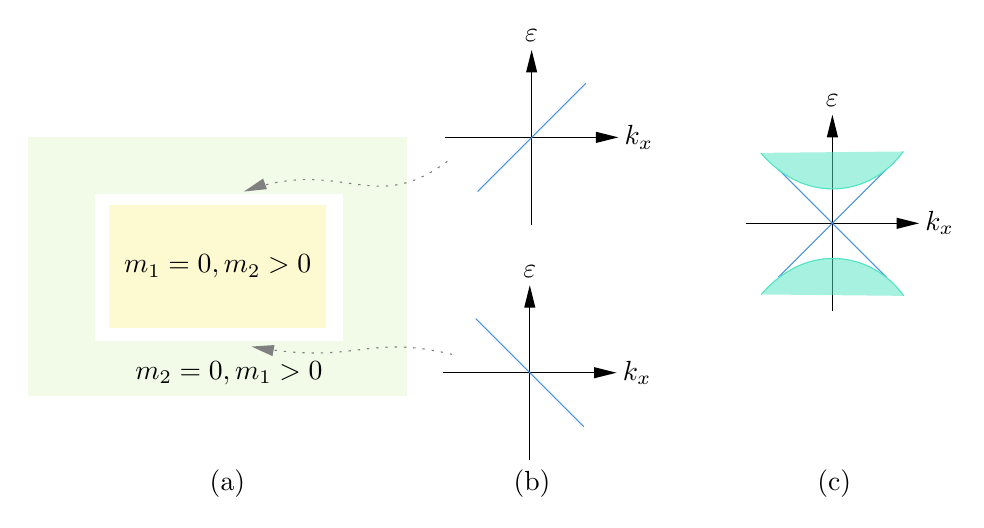
\begin{tikzpicture}[x=0.75pt,y=0.75pt,yscale=-0.9,xscale=0.9]
    %uncomment if require: \path (0,300); %set diagram left start at 0, and has height of 300
    
    %Shape: Rectangle [id:dp47381136392650935] 
    \draw  [draw opacity=0][fill={rgb, 255:red, 184; green, 233; blue, 134 }  ,fill opacity=0.2 ] (119.5,85.88) -- (322.33,85.88) -- (322.33,224.69) -- (119.5,224.69) -- cycle ;
    %Shape: Rectangle [id:dp4339114151270278] 
    \draw  [draw opacity=0][fill={rgb, 255:red, 255; green, 255; blue, 255 }  ,fill opacity=1 ] (155,116.38) -- (287.83,116.38) -- (287.83,195.05) -- (155,195.05) -- cycle ;
    %Shape: Rectangle [id:dp2989871396977255] 
    \draw  [draw opacity=0][fill={rgb, 255:red, 248; green, 231; blue, 28 }  ,fill opacity=0.2 ] (163,122.38) -- (278.83,122.38) -- (278.83,188.19) -- (163,188.19) -- cycle ;
    %Straight Lines [id:da6228043720397025] 
    \draw    (342.58,86.02) -- (433.42,86.02) ;
    \draw [shift={(435.42,86.02)}, rotate = 180] [fill={rgb, 255:red, 0; green, 0; blue, 0 }  ][line width=0.08]  [draw opacity=0] (12,-3) -- (0,0) -- (12,3) -- cycle    ;
    %Straight Lines [id:da1342683118643182] 
    \draw    (389,132.85) -- (389,41.19) ;
    \draw [shift={(389,39.19)}, rotate = 90] [fill={rgb, 255:red, 0; green, 0; blue, 0 }  ][line width=0.08]  [draw opacity=0] (12,-3) -- (0,0) -- (12,3) -- cycle    ;
    %Curve Lines [id:da9897885979824663] 
    \draw [color={rgb, 255:red, 128; green, 128; blue, 128 }  ,draw opacity=1 ] [dash pattern={on 0.84pt off 2.51pt}]  (237.35,114.17) .. controls (288.32,96.83) and (304.43,128.4) .. (343.83,98.85) ;
    \draw [shift={(235,115)}, rotate = 340.08] [fill={rgb, 255:red, 128; green, 128; blue, 128 }  ,fill opacity=1 ][line width=0.08]  [draw opacity=0] (12,-3) -- (0,0) -- (12,3) -- cycle    ;
    %Straight Lines [id:da4087737798695412] 
    \draw    (341.58,212.02) -- (432.42,212.02) ;
    \draw [shift={(434.42,212.02)}, rotate = 180] [fill={rgb, 255:red, 0; green, 0; blue, 0 }  ][line width=0.08]  [draw opacity=0] (12,-3) -- (0,0) -- (12,3) -- cycle    ;
    %Straight Lines [id:da9829350008771554] 
    \draw    (388,258.85) -- (388,167.19) ;
    \draw [shift={(388,165.19)}, rotate = 90] [fill={rgb, 255:red, 0; green, 0; blue, 0 }  ][line width=0.08]  [draw opacity=0] (12,-3) -- (0,0) -- (12,3) -- cycle    ;
    %Straight Lines [id:da8956046655127317] 
    \draw [color={rgb, 255:red, 74; green, 144; blue, 226 }  ,draw opacity=1 ]   (359.08,183.1) -- (416.92,240.94) ;
    %Straight Lines [id:da8044896844364018] 
    \draw [color={rgb, 255:red, 74; green, 144; blue, 226 }  ,draw opacity=1 ]   (417.92,57.1) -- (360.08,114.94) ;
    %Curve Lines [id:da16545040495133922] 
    \draw [color={rgb, 255:red, 128; green, 128; blue, 128 }  ,draw opacity=1 ] [dash pattern={on 0.84pt off 2.51pt}]  (241.57,198.45) .. controls (296.9,207.99) and (299.57,190.7) .. (347.83,202.52) ;
    \draw [shift={(239,198)}, rotate = 10.31] [fill={rgb, 255:red, 128; green, 128; blue, 128 }  ,fill opacity=1 ][line width=0.08]  [draw opacity=0] (12,-3) -- (0,0) -- (12,3) -- cycle    ;
    %Straight Lines [id:da06617989023995818] 
    \draw    (503.58,132.02) -- (594.42,132.02) ;
    \draw [shift={(596.42,132.02)}, rotate = 180] [fill={rgb, 255:red, 0; green, 0; blue, 0 }  ][line width=0.08]  [draw opacity=0] (12,-3) -- (0,0) -- (12,3) -- cycle    ;
    %Straight Lines [id:da7325772285954404] 
    \draw    (550,178.85) -- (550,75.97) ;
    \draw [shift={(550,73.97)}, rotate = 90] [fill={rgb, 255:red, 0; green, 0; blue, 0 }  ][line width=0.08]  [draw opacity=0] (12,-3) -- (0,0) -- (12,3) -- cycle    ;
    %Straight Lines [id:da010258872926008689] 
    \draw [color={rgb, 255:red, 74; green, 144; blue, 226 }  ,draw opacity=1 ]   (578.92,103.1) -- (521.08,160.94) ;
    %Straight Lines [id:da8638013572760861] 
    \draw [color={rgb, 255:red, 74; green, 144; blue, 226 }  ,draw opacity=1 ]   (521.08,103.1) -- (578.92,160.94) ;
    %Curve Lines [id:da3647571238097487] 
    \draw [color={rgb, 255:red, 80; green, 227; blue, 194 }  ,draw opacity=1 ][fill={rgb, 255:red, 80; green, 227; blue, 194 }  ,fill opacity=0.5 ]   (511.71,94.32) .. controls (535.96,122.82) and (570.96,117.32) .. (587.96,93.57) ;
    %Curve Lines [id:da8419595301038851] 
    \draw [color={rgb, 255:red, 80; green, 227; blue, 194 }  ,draw opacity=1 ][fill={rgb, 255:red, 80; green, 227; blue, 194 }  ,fill opacity=0.5 ]   (511.96,170.11) .. controls (536.21,141.61) and (571.21,147.11) .. (588.21,170.86) ;
    
    % Text Node
    \draw (220.92,155.28) node    {$m_{1} =0,m_{2}  >0$};
    % Text Node
    \draw (226.92,212.09) node    {$m_{2} =0,m_{1}  >0$};
    % Text Node
    \draw (437.42,86.02) node [anchor=west] [inner sep=0.75pt]    {$k_{x}$};
    % Text Node
    \draw (389,36.19) node [anchor=south] [inner sep=0.75pt]    {$\varepsilon $};
    % Text Node
    \draw (436.42,212.02) node [anchor=west] [inner sep=0.75pt]    {$k_{x}$};
    % Text Node
    \draw (388,162.19) node [anchor=south] [inner sep=0.75pt]    {$\varepsilon $};
    % Text Node
    \draw (598.42,132.02) node [anchor=west] [inner sep=0.75pt]    {$k_{x}$};
    % Text Node
    \draw (550,70.97) node [anchor=south] [inner sep=0.75pt]    {$\varepsilon $};
    % Text Node
    \draw (215.22,262.79) node [anchor=north west][inner sep=0.75pt]   [align=left] {(a)};
    % Text Node
    \draw (377.89,262.79) node [anchor=north west][inner sep=0.75pt]   [align=left] {(b)};
    % Text Node
    \draw (540.56,262.79) node [anchor=north west][inner sep=0.75pt]   [align=left] {(c)};
    
    
    \end{tikzpicture}
    